\section{Epidemiological modeling of rumors}
Another way to study the spread of rumors (versus news) is from an epidemiological modeling standpoint. An epidemiological model helps capture the likelihood of an individual getting infected with a virus or, here, of adopting an idea that he or she has been exposed to.

\begin{figure}[ht]
\centering
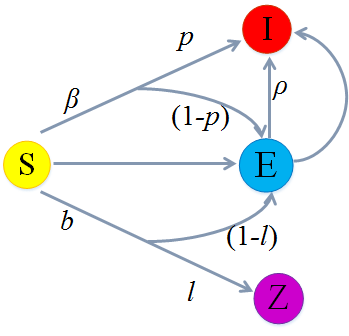
\includegraphics[width=2in]{pictures/SEIZ.png} %?????????????
\caption{The SEIZ compartmental model. The various states denote: (S) Susceptible. (I) Infected. (E) Exposed. (Z) Skeptic.}
\label{fig:Ebola_SEIZ_raw}
\end{figure}

In earlier work~\cite{jin2013epidemiological} we demonstrated how we can accomplish this objective using the SEIZ epidemiological model that was originally proposed to study the adoption of ideas~\cite{powerofgoodidea:2006}. The SEIZ model is particularly suited to studying rumor propagation as it captures distinctions in how people respond to ideas: whether they adopt it readily or are initially skeptical.

The idea in the SEIZ model is to compartmentalize a population into four categories, denoted as S, E, I, and Z. We interpret these categories with specific reference to Twitter propagation. Susceptible (S) represents a user who has not heard the information; infected (I) denotes a user who has (re)tweeted about the information; skeptic (Z) denotes a user who has heard about the information but chooses not to (re)tweet about it; and exposed (E) represents a user who has received the information via a tweet but has taken some time, an exposure delay, prior to reposting or sharing that information.

\begin{figure}[ht]
\centering
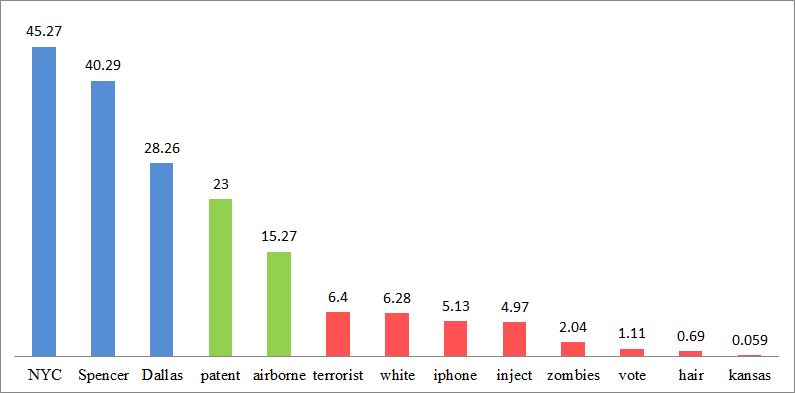
\includegraphics[width=5in]{pictures/R_si_values.png} %?????????????
\caption{Response ratios for 3 news stories (left) and 10 rumors related to Ebola.}
\label{fig:Ebola_response_ratio}
\end{figure}


The transitions between these states are modeled as shown in Fig~\ref{fig:Ebola_SEIZ_raw}. We caution that referring to the Z compartment as a �skeptic� is in no way an implication of the underlying truth or falsehood of the information; it simply helps capture whether users readily adopt an idea or take some time to adopt it.

Model fits of SEIZ to the different rumors and time course information for each of the state variables is given in Figure~\ref{fig:Ebola_SEIZ_fitting}. As can be seen the SEIZ model is capable of capturing a variety of information spread patterns: quasi-linear (e.g., �patent�), sigmoidal (�white�), and other non-linear patterns (�zombies� and �airborne�).


\begin{figure}[th]
\centering
\subfigure[white]{
   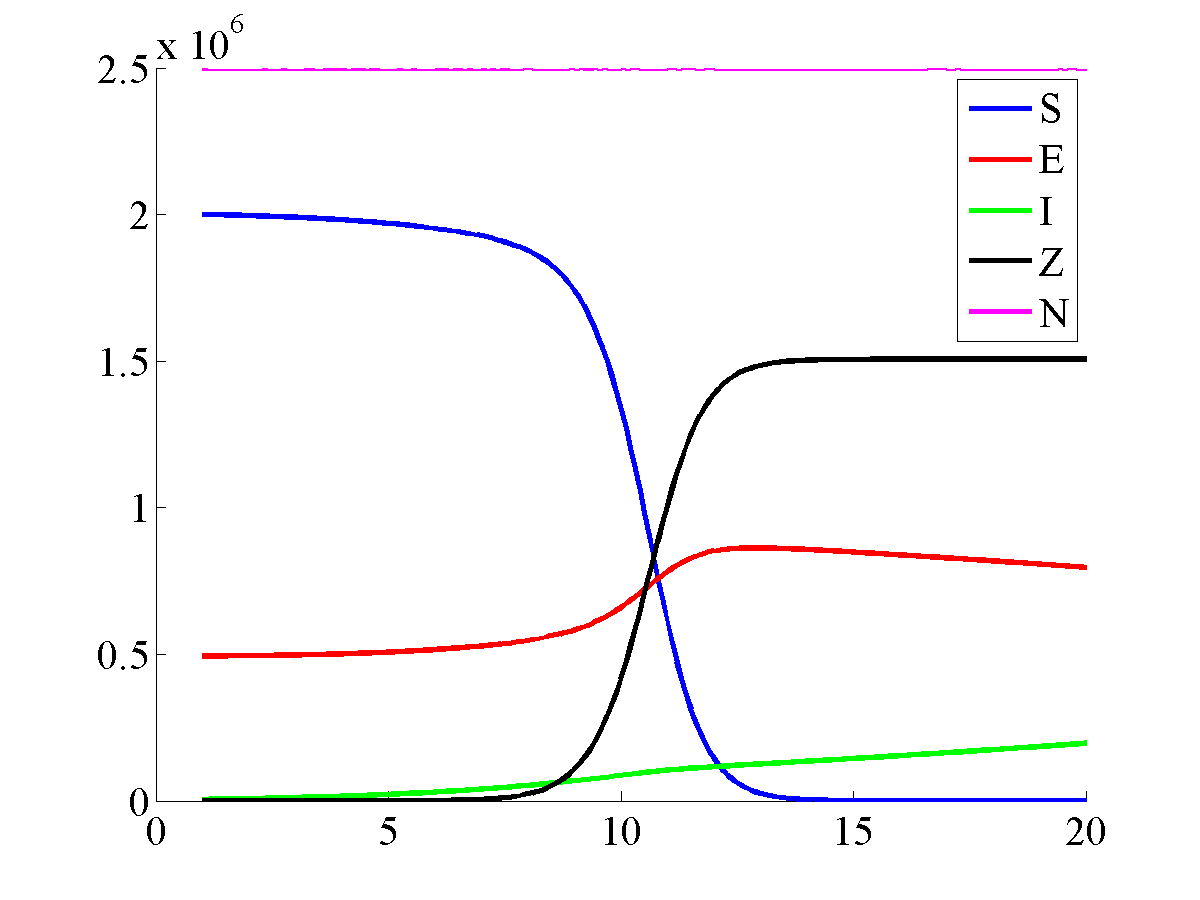
\includegraphics[width=1.45in] {pictures/b-white_SEIZ_timecourse.png}
  \label{fig:b-white_SEIZ_timecourse}
 }
 \subfigure[zombies]{
   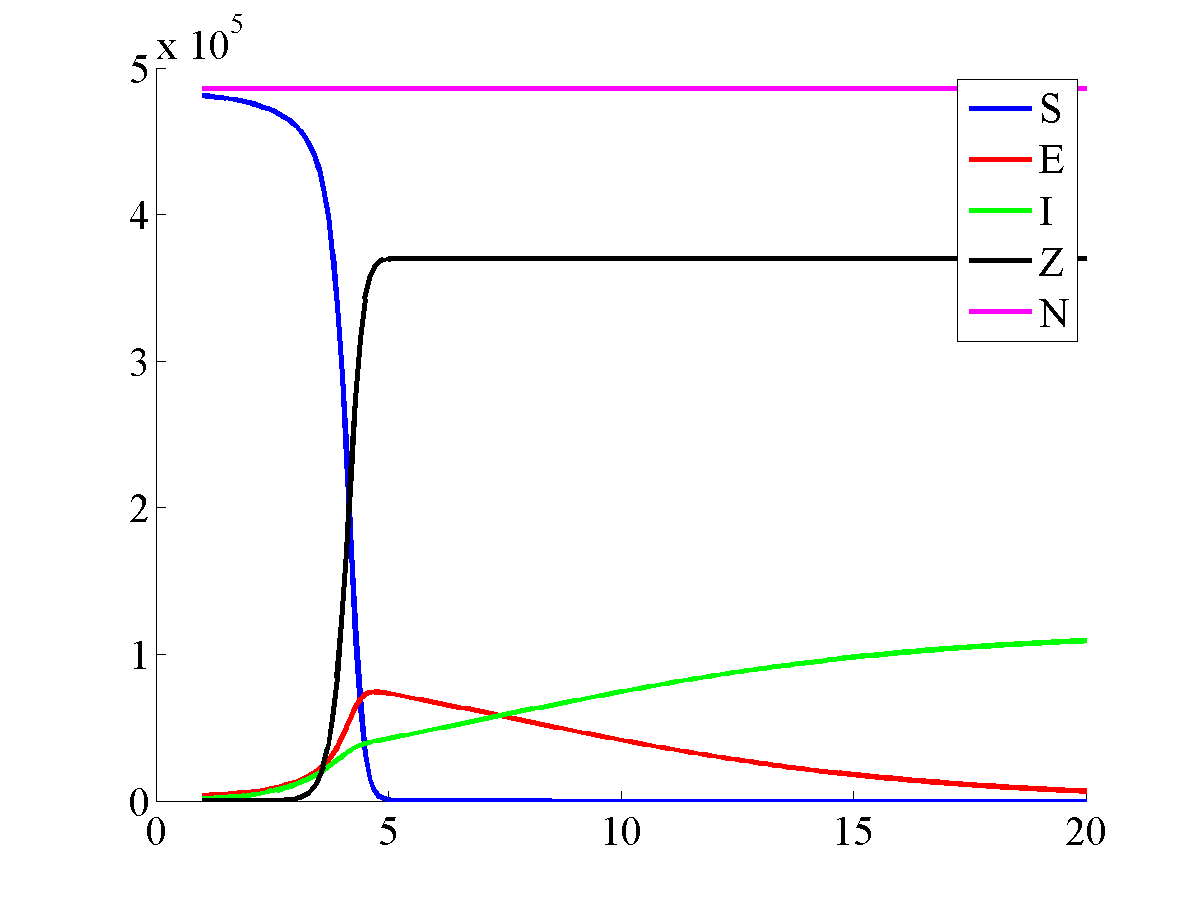
\includegraphics[width=1.45in] {pictures/c-zombies_SEIZ_timecourse.png}
  \label{fig:c-zombies_SEIZ_timecourse}
 }
 \subfigure[airborne]{
   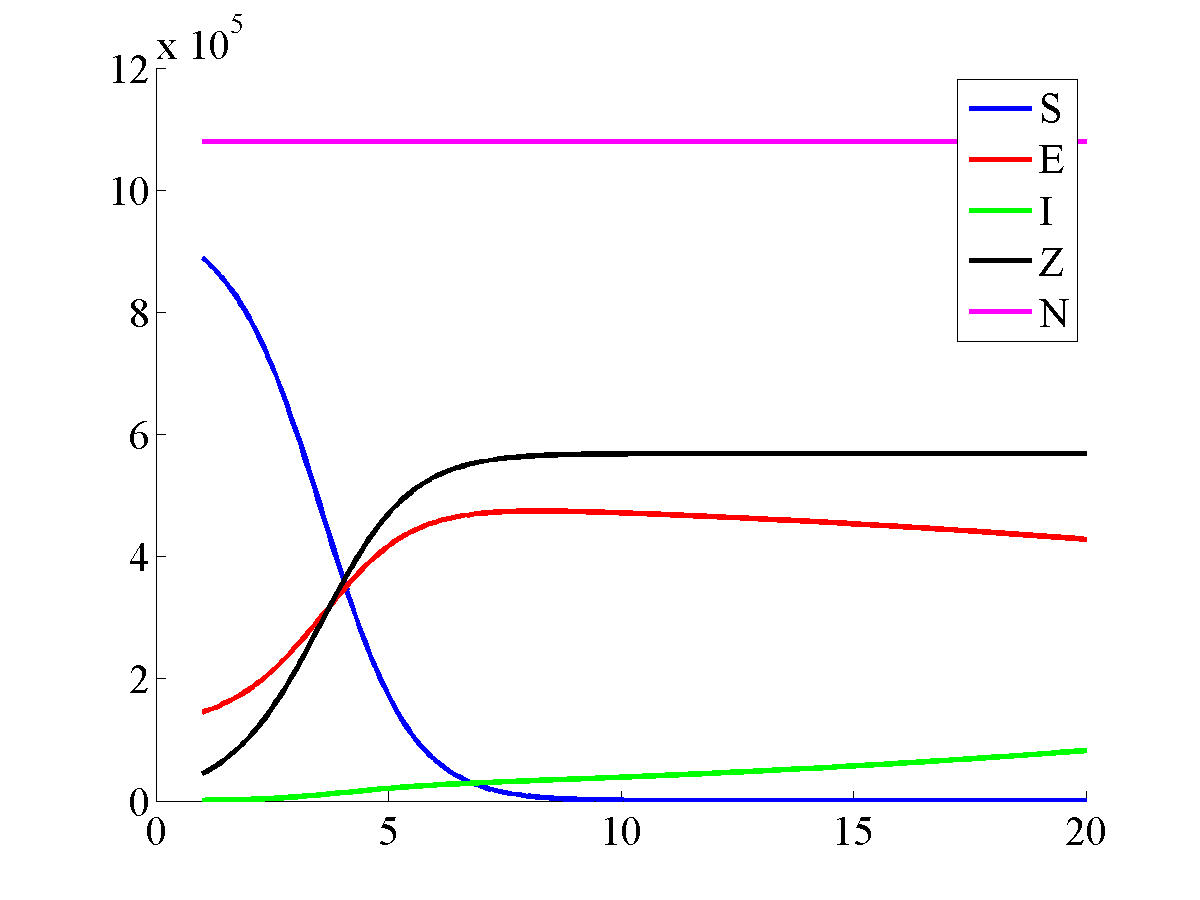
\includegraphics[width=1.45in] {pictures/d-airborne_SEIZ_timecourse.png}
  \label{fig:d-airborne_SEIZ_timecourse}
 }
  \subfigure[patent]{
   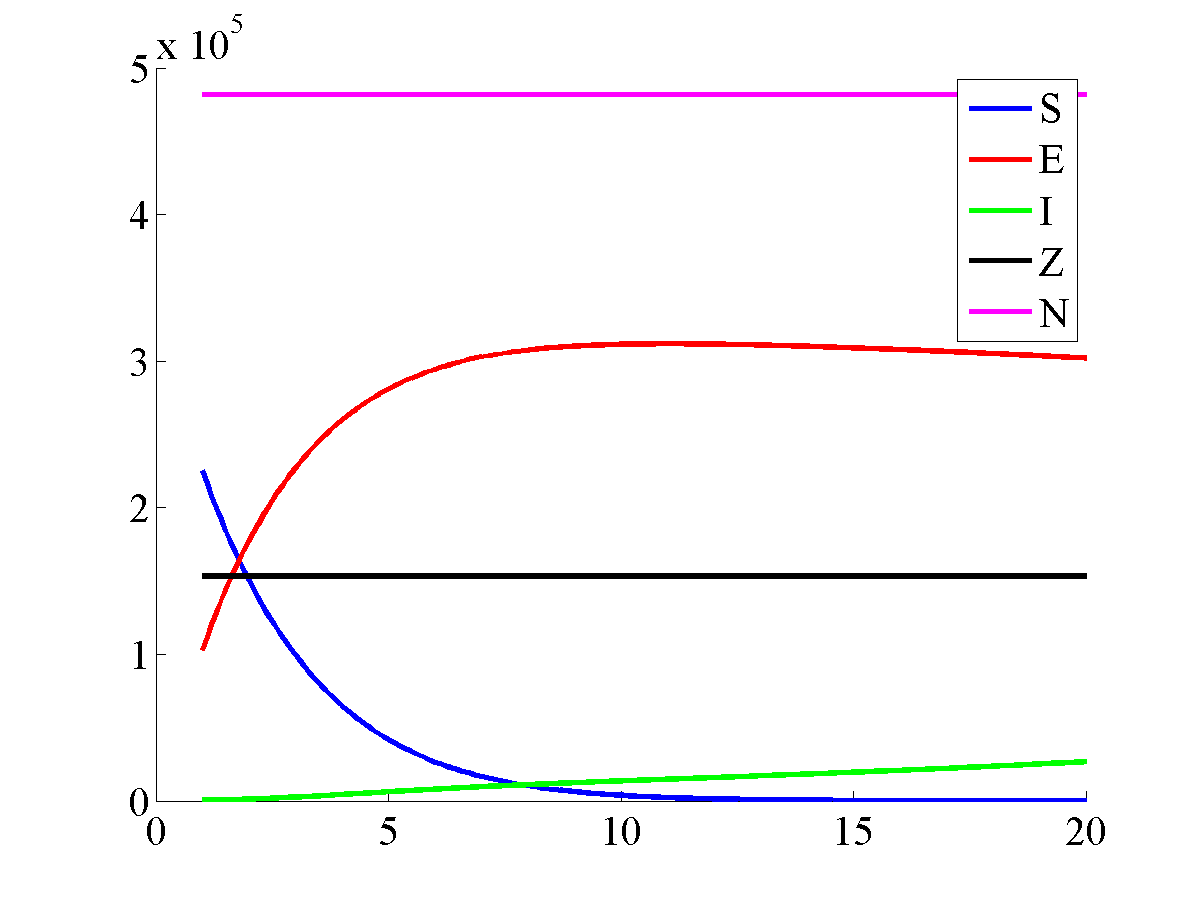
\includegraphics[width=1.45in] {pictures/e-patent_SEIZ_timecourse.png}
  \label{fig:e-patent_SEIZ_timecourse}
 }
 \subfigure[white]{
   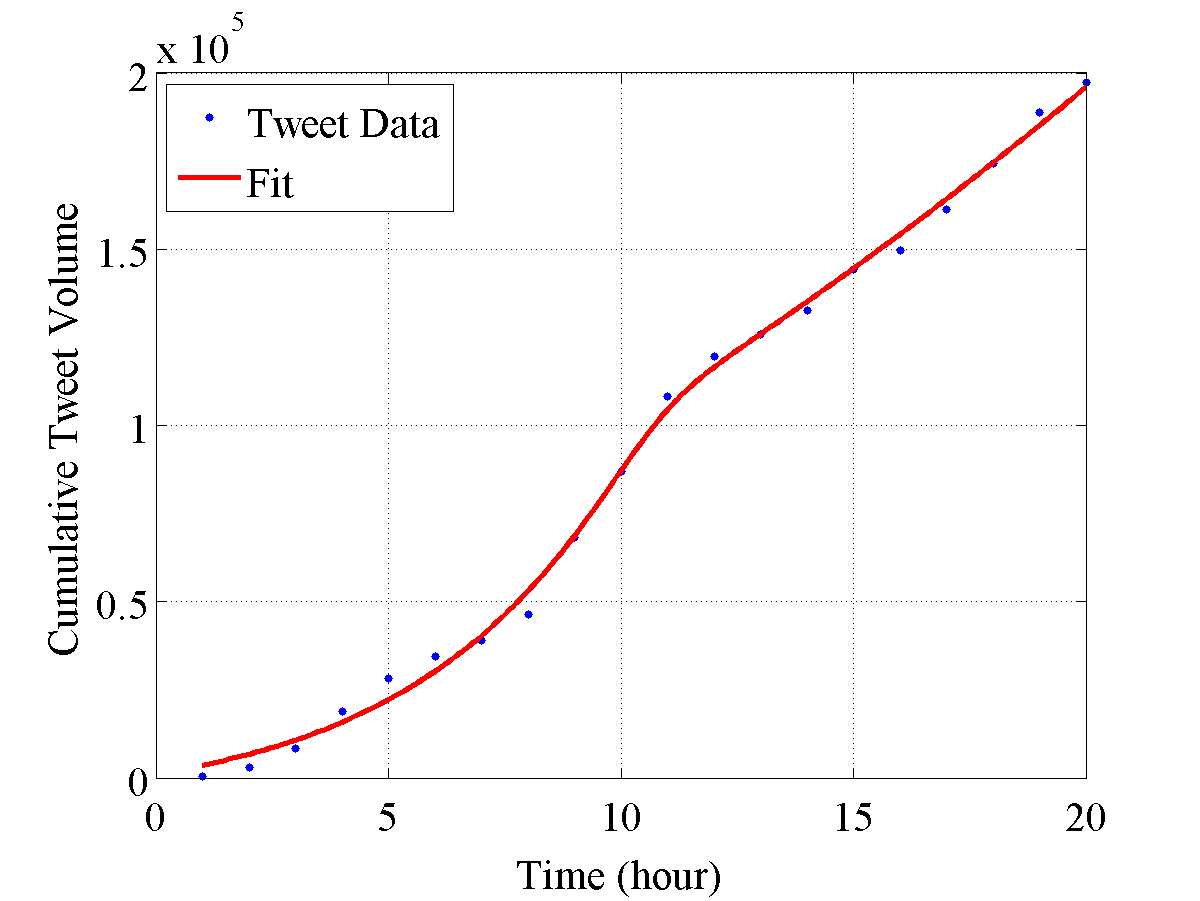
\includegraphics[width=1.45in] {pictures/Fig7-white-fitting.png}
  \label{fig:Ebola-white-fitting}
 }
 \subfigure[zombies]{
   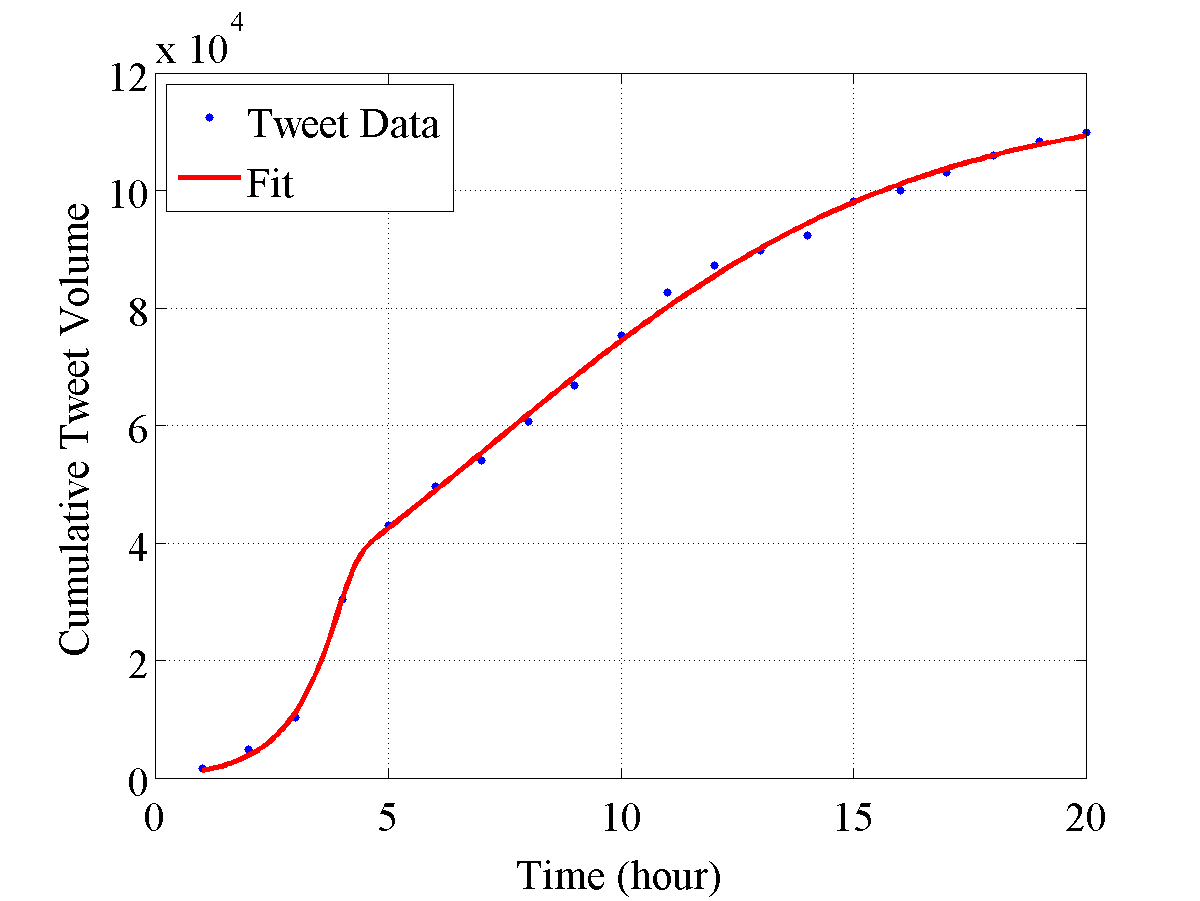
\includegraphics[width=1.45in] {pictures/Fig7-zombies-fitting.png}
  \label{fig:Ebola-zombies-fitting}
 }
 \subfigure[airborne]{
   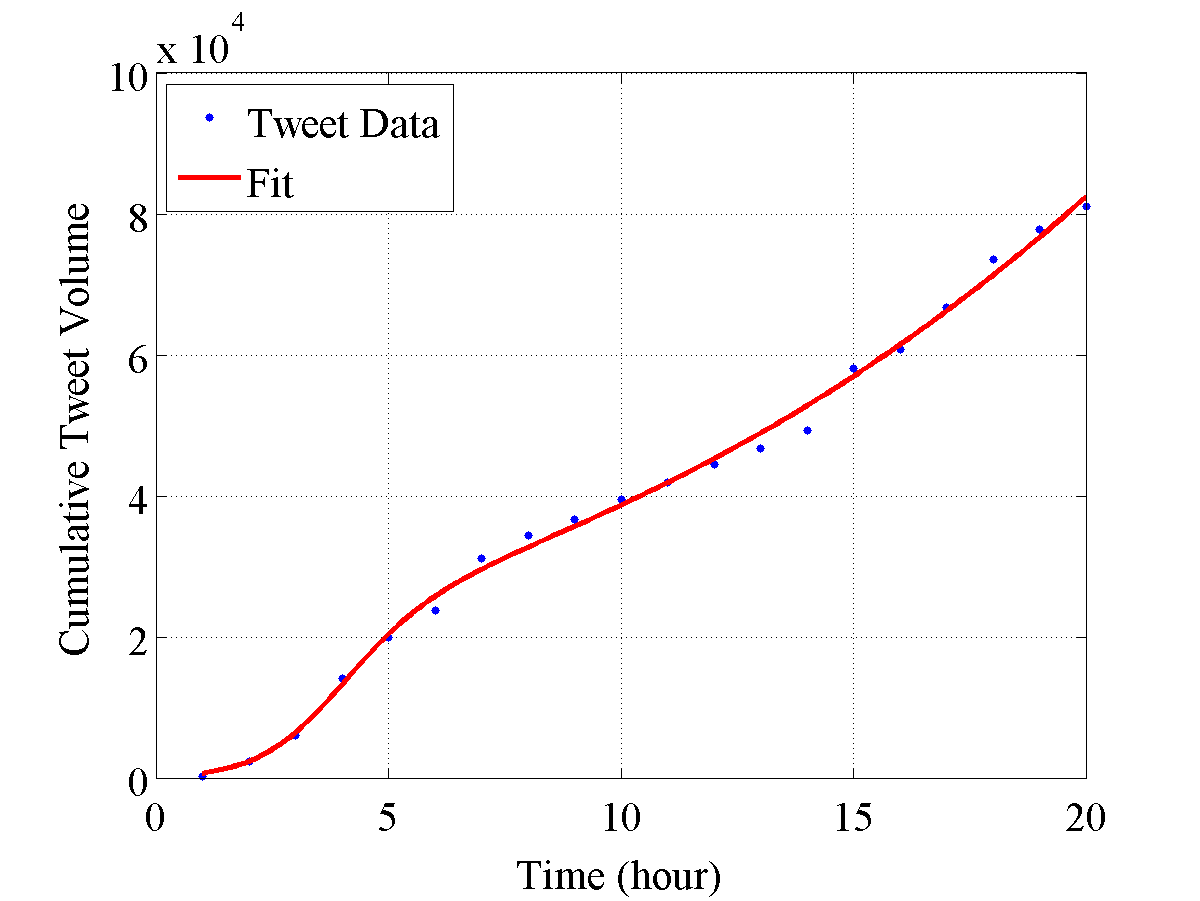
\includegraphics[width=1.45in] {pictures/Fig7-airborne-fitting.png}
  \label{fig:Ebola-airborne-fitting}
 }
  \subfigure[patent]{
   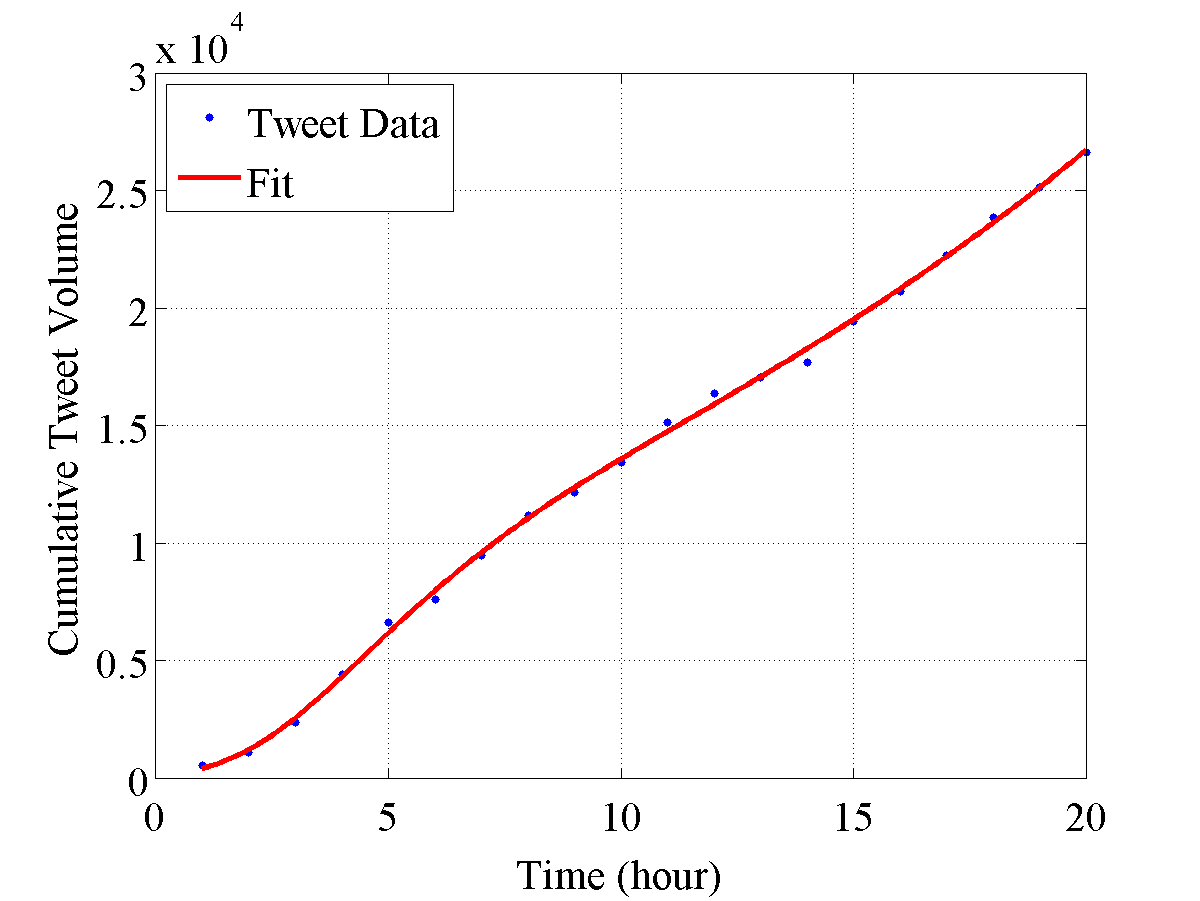
\includegraphics[width=1.48in] {pictures/Fig7-patent-fitting.png}
  \label{fig:Ebola-patent-fitting}
 }
\caption{Model fits of SEIZ to different rumors: (from left to right) �white�, �zombies�, �airborne�, and �patent�. (top row) Fitting results. (bottom row) time-course profiles of different compartments. }
\label{fig:Ebola_SEIZ_fitting}
\end{figure}

Time course results from the SEIZ compartmental model as shown in Figure~\ref{fig:Ebola_SEIZ_fitting} depict broadly similar patterns. Here �N� denotes the total size of the population (distinct Twitter users). High values of S rapidly decrease with a relatively comparable increase in Z, and a gradual increase in I that continues as E decreases. However, the patent rumor time-course data has a noticeably different response profile than the other rumor examples.

Here, the initial value of the S group begins with less than half of the total population size, and only slightly higher than the initial values of the Z and E groups. Second, the Z group is essentially constant, meaning that the number of skeptics does not change throughout the propagation time course. Third, the decrease in S does not correspond to a change in Z, as is observed in the other rumor examples. Rather, the drop in S is met with a near identical increase in E.


These findings hint that a large influx into E without a corresponding efflux to I combined with a stagnant Z group will produce an elevated response ratio. In other words, there is a large exposure to the rumor topic without significant change in skepticism.

In our earlier work on characterizing rumors~\cite{jin2013epidemiological}, we defined the notion of a �response ratio� which quantifies transitions through the exposed compartment. The response ratio provides a relative measure of the population influx into the E compartment versus the efflux from this compartment. We hypothesize that this ratio could be one of the factors useful in discriminating rumors from true news, with larger response ratios associated with factual news topics.

To compare response ratios across rumor and news, we select three breaking (true) news stories pertaining to Ebola: `Dallas' refers to the story of the first Ebola patient (Duncan) identified in the US; `NYC' refers to the first confirmation of an Ebola patient (Spencer) in New York City; and `Spencer' refers to the specific symptoms and travel activities of Spencer in the days before he was diagnosed.

The response ratios for these three news stories and other rumors are shown in Figure~\ref{fig:Ebola_response_ratio}. It can be seen that all three news stories (blue bars) have response ratios higher than 25, with a mean value of approximately 38, while eight of the 10 rumors stories (red bars) have a response ratio less than or equal to 6.4, with a mean of only 3.33. Two of the 10 rumors (green bars; `paten' and `airborne') have elevated response values, suggesting that there was greater belief associated with these topics than the other eight rumors.

The study here has shown that propagation of misinformation can sometimes have the same characteristics as genuine newsworthy developments.  In an age where many consumers receive their news from real-time social media platforms, it is imperative that rumors and half-truths be characterized as such and able to be distinguished from news. The tools presented here can support the quantitative evaluation of information spread as it happens.
